%GiG
\documentclass{beamer} 
\usetheme{Copenhagen}
\setbeamertemplate{navigation symbols}{}
\setbeamertemplate{headline}{}
\DeclareMathOperator*{\argmax}{arg\,max}

\usepackage{hyperref}


\definecolor{azure}{rgb}{0.0, 0.5, 1.0}
%\newcommand{\tblue}[1]{\textcolor{blue}{#1}}
\newcommand{\tblue}[1]{{\Large {\textcolor{azure}{#1}}}}
\newcommand{\thblue}[1]{{\Huge {\textcolor{azure}{#1}}}}
\newcommand{\hred}[1]{{\textcolor{red}{#1}}}
\newcommand{\furl}[1]{{\footnote{\url{#1}}}}

\newcommand{\mypause}{\pause}
%\newcommand{\mypause}{}

\title[Saravanan Thirumuruganathan] 
{Lecture 6: $k$-Nearest Neighbors}

\author[CSE 5334] 
{Instructor: Saravanan Thirumuruganathan}

\date[] 

\begin{document}


\begin{frame}
  \titlepage
\end{frame}

%\begin{frame}{Outline}
%  \tableofcontents
%  % You might wish to add the option [pausesections]
%\end{frame}

\section{Outline}

\begin{frame}
\frametitle {Outline}
\begin{enumerate}
\item Introduction to Classification
\item $k$-NN (Nearest Neighbor) Classifier
\end{enumerate}
\end{frame}


\begin{frame}{In-Class Quizzes}
\begin{itemize}
\item {\Large {\bf URL:}} {\LARGE \bf \url{http://m.socrative.com/}} 
\item {\Large {\bf Room Name:} {\LARGE \bf 4f2bb99e}}
\end{itemize}
\end{frame}


\section{Data Mining}
\begin{frame}{} 
    \begin{center}
        \thblue{Introduction to Classification}
    \end{center}
\end{frame}

\begin{frame}{Major Tasks in Data Mining}
    \begin{itemize}
        \item Predictive methods
            \begin{itemize}
                \item Given some training data, build a model and use it to predict some variables of interest for unseen data  
            \end{itemize}
        \item Descriptive methods
            \begin{itemize}
                \item Given some data, identify some significant, novel and useful patterns in the data that are interpretable by humans
            \end{itemize}
    \end{itemize}
\end{frame}

\begin{frame}{Data Mining Tasks}
    \begin{itemize}
        \item Classification, Regression: Predictive
        \item Clustering, Association Rule mining: Descriptive
    \end{itemize}
\end{frame}

\begin{frame}{Types of Learning}
    \begin{itemize}
        \item Supervised Learning 
        \item Unsupervised Learning
        \item Reinforcement Learning
    \end{itemize}
\end{frame}


\begin{frame}{Supervised Learning}
    \begin{itemize}
        \item {\bf Dataset:} 
        \begin{itemize}
            \item \hred{Training} (labeled) data: $D = \{ (x_i, y_i) \}$
            \item $x_i \in \mathbb{R}^d$
            \item \hred{Test} (unlabeled) data: $x_0 \in \mathbb{R}^d$
        \end{itemize}
        \item {\bf Tasks:}
        \begin{itemize}
            \item Classification: $y_i \in \{1, 2, \ldots, C\}$
            \item Regression: $y_i \in \mathbb{R}$
        \end{itemize}
        \item {\bf Objective:} Given $x_0$, predict $y_0$
        \item {\bf Supervised} learning as $y_i$ was given during training
    \end{itemize}
\end{frame}


\begin{frame}{Unsupervised Learning}
    \begin{itemize}
        \item Given: dataset $D = \{x_i\}$
        \item Objective: Find interesting patterns without explicit supervision
        \item {\bf Tasks:}
        \begin{itemize}
            \item Clustering
            \item Outlier detection
            \item Dimensionality reduction
            \item Many more
        \end{itemize}
    \end{itemize}
\end{frame}


\begin{frame}{Reinforcement Learning}
    \begin{itemize}
        \item Training ``agents'' to take actions to maximize rewards
        \item Reinforcement is given via action-reward
        \item Objective: Find out what is the optimal action {\bf a} to take when in state {\bf x}, in order to maximize long-term reward
        \item {\bf Examples:} Learning correct answers from score, self-driving cars, learning to fly helicopters autonomously, learning to play games
    \end{itemize}
\end{frame}


\begin{frame}{Classification Methods}
    \begin{itemize}
        \item {\bf Model based:} Build a (simple) model from the training data and use it to predict unseen data
        \item {\bf Memory based:} Keep in memory all training data and use it to predict unseen data
    \end{itemize}
\end{frame}


\begin{frame}{Classification Models}

    Some of the methods we will discuss in the class:
    \begin{itemize}
        \item Tree based: Decision and Regression trees
        \item Instance based: Nearest Neighbor 
        \item Bayesian and Naive Bayes
        \item Neural Networks and Deep Learning
        \item Support Vector Machines
    \end{itemize}
\end{frame}

\begin{frame}{Binary and Multi-Class Classification}
    \begin{itemize}
        \item $C=2$: Predict which of the two classes for the unseen record 
        \begin{itemize}
            \item Spam or Ham for emails
            \item Benign or malignant for tumours
        \end{itemize}
        \item $C > 2$: Multi-Class classification - predict the right class.
        \begin{itemize}
            \item Categorize mail as important, social, unimportant
            \item Identify color of eyes
            \item Identify wine type from features
        \end{itemize}
        \item Multi-class classification is often much more harder
    \end{itemize}
\end{frame}

\begin{frame}{Trade-offs}
    \begin{itemize}
        \item Prediction accuracy versus interpretability
        \item Good fit versus over-fit or under-fit
        \item Parsimony versus black-box
    \end{itemize}
\end{frame}

\begin{frame}{Classification Design Cycle\furl{http://www.cs.sun.ac.za/~kroon/courses/machine_learning/lecture2/kNN-intro_to_ML.pdf}}
    \begin{enumerate}
        \item Collect data and labels (the real effort)
        \item Choose features (the real ingenuity)
        \item Pick a classifier (some ingenuity)
        \item Train the classifier (some knobs, fairly mechanical)
        \item Evaluate the classifier (needs care)
    \end{enumerate}
\end{frame}

\section{$k$-NN Classifier}
\begin{frame}{} 
    \begin{center}
        \thblue{$k$-NN Classifier}
    \end{center}
\end{frame}

\begin{frame}{Instance based Classifiers}
    \begin{itemize}
        \item Store ALL the training data 
        \item Use the training data to predict class label for a new record
        \item Common Examples:
        \begin{itemize}
            \item Rote-Learner: Memorize entire training data, predict value if the new record matches some training data
            \item Nearest Neighbor: Use $k$ points closest to new record to perform classification
        \end{itemize}
    \end{itemize}
\end{frame}


\begin{frame}{Nearest Neighbor Methods}
    \begin{itemize}
        \item Non-parametric, model-free approaches
        \item Formalized in 1960s
        \item Simple to understand and implement
    \end{itemize}
\end{frame}


\begin{frame}{Why $k$-NN}
    \begin{itemize}
        \item One of the top-10 Data Mining algorithms\furl{http://www.cs.umd.edu/~samir/498/10Algorithms-08.pdf}
        \item {\bf $1$-NN Error bounds:} 
        \begin{itemize}
            \item When number of training data $n$ tends to $\infty$ in a $C$-Class problem then the $1$-NN error rate (1NNER) 
                is bounded by $$BER \leq 1NNER \leq BER \times \left( 2 - \frac{C}{C-1} \times BER \right)$$
            \item $1$-NN Error rate is at most twice that of BER
        \end{itemize}
        \item Asymptotically Consistent: With infinite training data and large enough $k$, $k$-NN approaches the best possible classifier (Bayes Optimal)
    \end{itemize}
\end{frame}


\begin{frame}{$k$-Nearest Neighbor}
    \begin{itemize}
        \item Distance Metric: To compute the similarities between records 
        \item $k$: How many neighbors to look at?
        \item A weighting function (optional)
        \item Decision strategy: Often simple majority voting
    \end{itemize}
\end{frame}


\begin{frame}{$k$-NN Algorithm}
    \begin{enumerate}
        \item Compute the test point's distance from each training point
        \item Sort the distances in ascending (or descending) order
        \item Use the sorted distances to select the $k$ nearest neighbors
        \item Use majority rule (for classification) or averaging (for regression)
    \end{enumerate}
\end{frame}


\begin{frame}{$1$-NN Example\furl{http://www.lkozma.net/knn2.pdf}}
    \begin{center}
        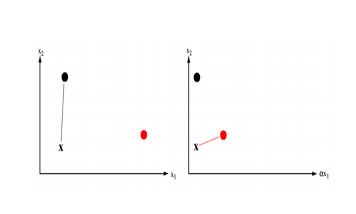
\includegraphics[scale=0.75]{1NN.png}
    \end{center}
\end{frame}

\begin{frame}{$k$-NN Example\furl{http://www.lkozma.net/knn2.pdf}}
    \begin{center}
        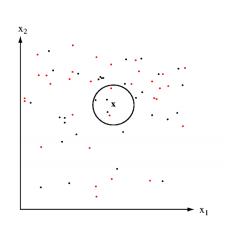
\includegraphics[scale=0.75]{kNN.png}
    \end{center}
\end{frame}


\begin{frame}{Distance Metric}
    \begin{itemize}
        \item Used to compute similarity between entities
        \item If all values are numeric, Euclidean measure is often used
    \end{itemize}
\end{frame}
\begin{frame}{Voronoi Cells in 2D\furl{http://www.lkozma.net/knn2.pdf}}
    \begin{center}
        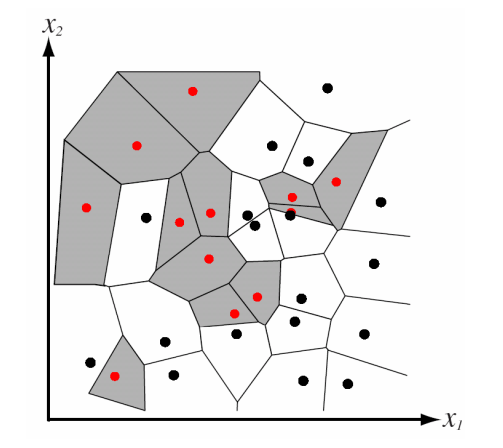
\includegraphics[scale=0.5]{voronoi2D.png}
    \end{center}
\end{frame}
\begin{frame}{Distance Metric}
    \begin{center}
        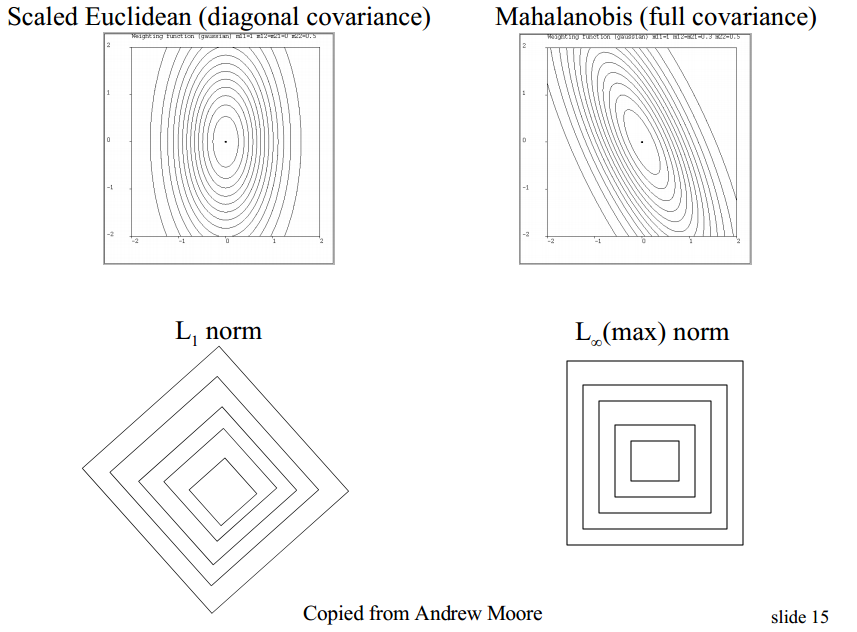
\includegraphics[scale=0.3]{distanceMetric.png}
    \end{center}
\end{frame}

\begin{frame}{Feature Normalization}
    \begin{itemize}
        \item Features should be on the {\bf same} scale
        \item Example: if one feature has its values in millimeters and another has in centimeters, we would need to normalize
        \item Common way: Center and Normalize to get $0$ mean and unit variance $$z_i = \frac{x_i - \overline{x_i}}{\sigma} $$
    \end{itemize}
\end{frame}


\begin{frame}{Finding Optimal $k$}
    \begin{itemize}
        \item Often $k$-NN has lower error rate than $1$-NN
        \item But the error does not monotonically decrease
        \item Picking $k$: Cross validation
    \end{itemize}
\end{frame}

\begin{frame}{Impact of $k$\furl{http://courses.cs.tamu.edu/rgutier/cs790_w02/l8.pdf}}
    \begin{center}
        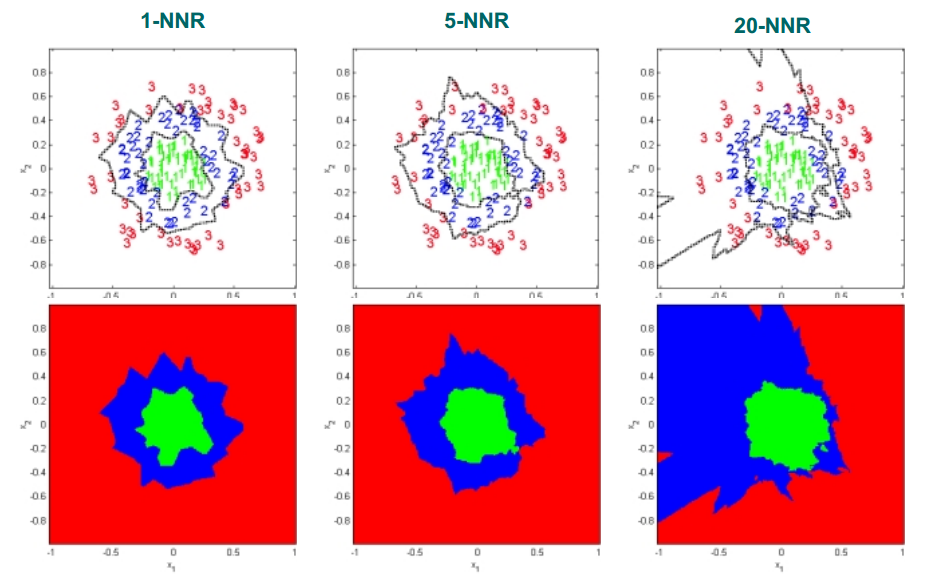
\includegraphics[scale=0.3]{varingK.png}
    \end{center}
\end{frame}
\begin{frame}{Impact of $k$\footnote{ISLR}}
    \begin{center}
        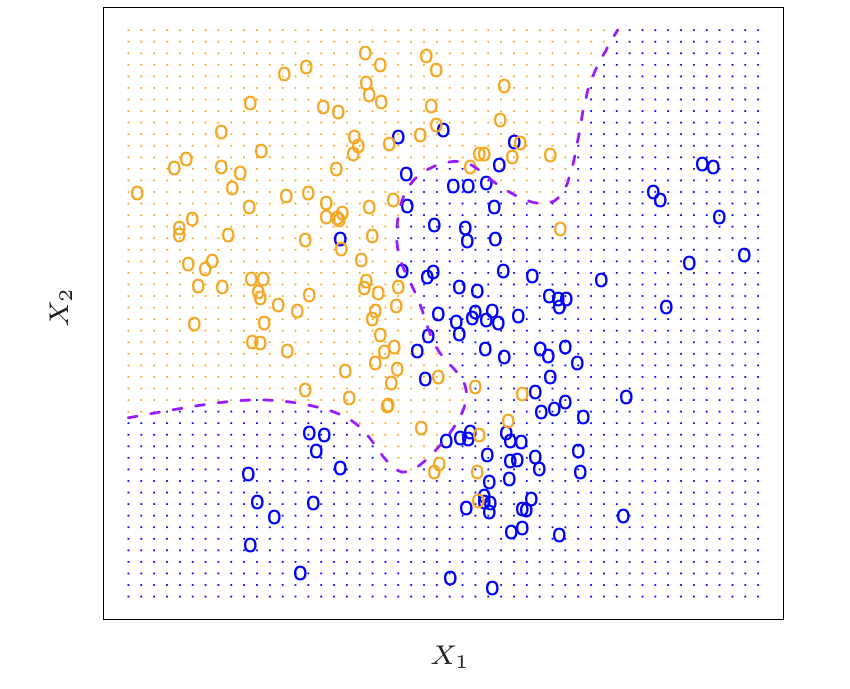
\includegraphics[scale=0.3]{knn2D.png}
    \end{center}
\end{frame}
\begin{frame}{Impact of $k$\footnote{ISLR}}
    \begin{center}
        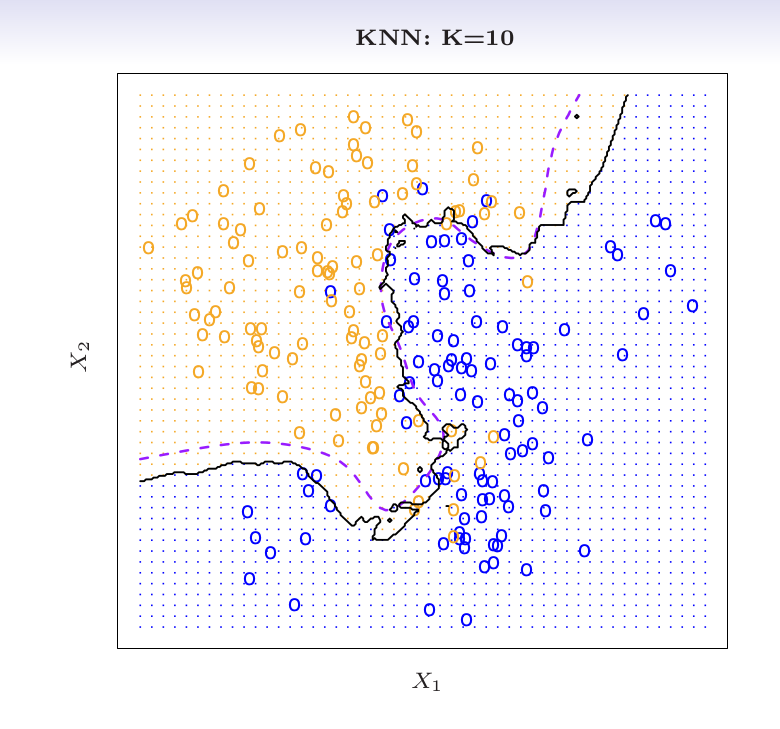
\includegraphics[scale=0.3]{knnK10.png}
    \end{center}
\end{frame}
\begin{frame}{Impact of $k$\footnote{ISLR}}
    \begin{center}
        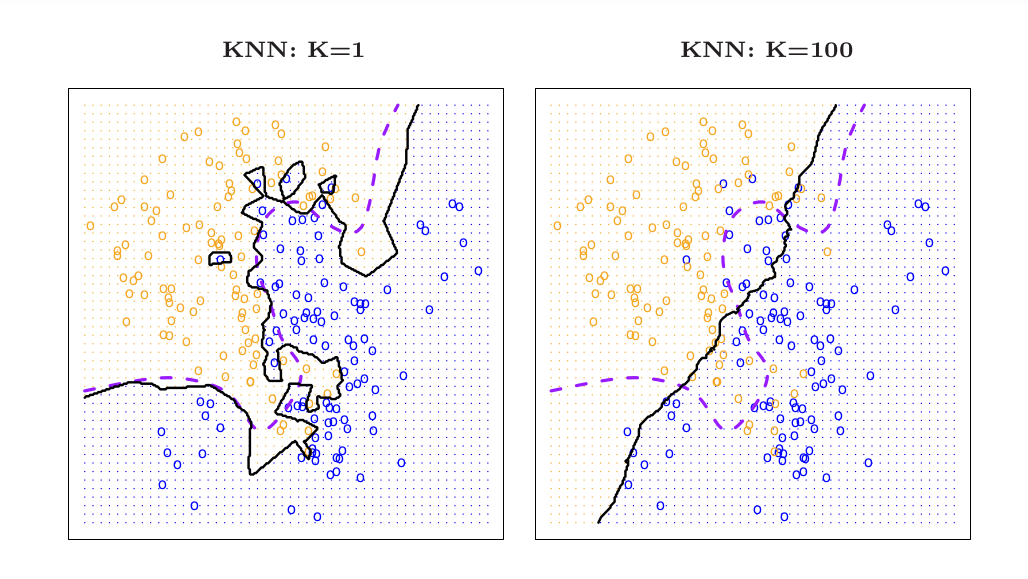
\includegraphics[scale=0.3]{knnK1K100.png}
    \end{center}
\end{frame}

\begin{frame}{Impact of $k$\furl{http://www.cs.cornell.edu/courses/CS4758/2013sp/materials/cs4758-knn-lectureslides.pdf}}
    \begin{itemize}
        \item Small $k$
            \begin{itemize}
                \item Creates many small regions for each class
                \item May lead to non-smooth decision boundaries and overfit
                \item Leads to higher variance (i.e. classifier is less stable)
            \end{itemize}
        \item Large $k$ 
            \begin{itemize}
                \item Creates fewer larger regions
                \item Usually leads to smoother decision boundaries (although, too smooth boundaries might underfit)
                \item Leads to higher bias (i.e. classifier is less precise)
            \end{itemize}
    \end{itemize}
\end{frame}

\begin{frame}{Weighted $k$-NN}
    \begin{itemize}
        \item Often you might want to use some weights
        \item Typically to give higher weights to points nearby than to points that are farther
        \item One possibility: $\frac{1}{dist^2}$ (i.e. inverse of squared distance)
        \item Alternatively, give more weight to similarity on important features $$dist(x_i, x_j) = \sum_{k=1}^{d} w_k \, dist(x_{ik}, x_{jk})$$
    \end{itemize}
\end{frame}




\begin{frame}{Computational Complexity}
    \begin{itemize}
        \item $O(nd)$ where $n$ is training set size and $d$ is the number of dimensions
        \item VERY expensive, computationally
        \item Often, special data structures such as Voronoi diagrams, KD-trees are used to speed things up.
    \end{itemize}
\end{frame}


\begin{frame}{Other Things to Watch Out}
    \begin{itemize}
        \item Missing data (features) will cause problems
        \item Sensitive to class outliers
        \item Sensitive to irrelevant features (so ensure feature engineering and normalization are done first)
    \end{itemize}
\end{frame}



\section{Summary}
\begin{frame}{Summary}

\tblue{Major Concepts:}
\begin{itemize}
    \item Major data mining tasks
    \item Classification basics
    \item $k$-NN, variants - pros and cons
\end{itemize}
\end{frame}

%\begin{frame}{Slide Material References}

%\begin{itemize}
%    \item 
%\end{itemize}
%\end{frame}


\end{document}

